\documentclass[useAMS,usenatbib,referee]{biom}

\usepackage{amsmath}
\usepackage[figuresright]{rotating}

\graphicspath{{../temp/rna-seq-stan/fig-rm-stan_laplace/}}

%%%%% PLACE YOUR OWN MACROS HERE %%%%%

\def\bSig\mathbf{\Sigma}
\newcommand{\VS}{V\&S}
\newcommand{\tr}{\mbox{tr}}

\title[eBayes for heterosis in RNAseq]{Empirical Bayes analysis for detection of gene heterosis in RNAseq data}

\author{Jarad Niemi $^*$\email{niemi@iastate.edu}, 
Eric Mittman, 
Will Landau, and 
Dan Nettleton \\
Department of Statistics, Iowa State University, Ames, Iowa, U.S.A.}

\begin{document}

\date{{\it Received December} 2014} 

\pagerange{\pageref{firstpage}--\pageref{lastpage}} 
\volume{VV}
\pubyear{YYYY}
\artmonth{Month}
\doi{x}

\label{firstpage}

%  put the summary for your paper here

\begin{abstract}
This is the summary for this paper.
\end{abstract}

\begin{keywords}
Empirical Bayes; Heterosis; Hierarchical Model; Negative binomial; RNAseq.
\end{keywords}

\maketitle

%  A maximum of six (6) tables or figures combined is often required.''

\section{Introduction}
\label{s:intro}

\section{Heterosis}
\label{s:heterosis}

\section{Empirical Bayes}
\subsection{Hierarchical model for RNAseq counts}
\label{s:model}

Let $Y_{gvi}$ be the count for gene $g=1,\ldots,F$, variety $v=1,\ldots,V$, and replicate $i=1,\ldots,n_v$. As shown in equation \eqref{e:data}, we assume a negative binomial for the counts with a mean that depends on the gene-variety combination through $\mu_{gv}$ and the sequencing depth $c_{vi}$ and a gene-specific over-dispersion $\psi_g$. Here $NB(\eta,\psi)$ indicates a negative-binomial with expectation $\eta$ and variance $\eta+\psi\eta^2$. 

\begin{equation} 
Y_{gvi} \stackrel{ind}{\sim} NB(e^{\mu_{gv}+\delta_{vi}},\psi_g) 
\label{e:data}
\end{equation}

A hierarchical model is constructed for the sequencing depth, overdispersion, and gene-variety parameters. The sample-specific sequencing depth terms are assumed to follow a normal distribution, i.e. $\delta_{vi} \stackrel{ind}{\sim} N(0,\tau_\delta^2)$. The logarithm of the gene-specific over-dispersion parameters also follow a normal distribution $\log(\psi_g) \stackrel{ind}{\sim} N(\zeta_\psi,\tau_\psi^2)$. The variety-specific effects for each gene, $\mu_g = (\mu_{g1},\ldots,\mu_{gV})'$ are assumed to have a joint normal distribution $\mu_g \stackrel{ind}{\sim} N(\eta, \Sigma)$. We consider an \emph{independent} model where $\Sigma$ is diagonal with elements $\sigma_1^2,\ldots,\sigma_V^2$ and a \emph{covariance} model where we estimate all parameters in $\Sigma$. 

We assume improper uniform priors for all hierarchical means and half-Cauchy priors for standard deviations, e.g. $\tau_\delta, \tau_\psi \stackrel{ind}{\sim} Ca^+(0,3)$ where 0 and 3 are the location and scale parameters on the untruncated distribution. In the independent model, we also assume $Ca^+(0,3)$ on the diagonal elements while in the covariance model, we assume a conjugate, proper inverse Wishart with degrees of freedom $V+1$ and an identity scale matrix. 

\subsection{Empirical Bayes}
\label{s:ebayes}

The parameters can be group by gene-specific parameters $\theta = (\theta_1,\ldots,\theta_G)$ and $\theta_g = (\mu_g,\psi_g)$ and non-gene-specific parameters $\phi = (\delta_{11},\ldots,\delta_{Vn_v}, \zeta_\psi, \tau_\psi^2, \Sigma)$. We employ an optimization procedure to obtain the \emph{maximum a posterior} (MAP) estimate for $\phi$, i.e. $\hat{\phi}_{MAP}$ and then base gene-specific inference on the posterior conditional on this estimated hyperparameter. Fortunately, conditional on the hyperparameters the gene specific parameters are conditionally independent as in equation \eqref{e:condind}. 

\begin{equation}
p(\theta|y,\hat{\phi}_{MAP}) = \prod_{g=1}^G p(\theta_g|y_g,\hat{\phi}_{MAP}) 
\label{e:condind}
\end{equation}

\section{Simulation study}
\label{s:simulation}

\subsection{Coverage for our model}

\input{../temp/analyze-heterosis/FIGURES/coverage}

\subsection{Heterosis detection}

\begin{figure}[htbp]
\centerline{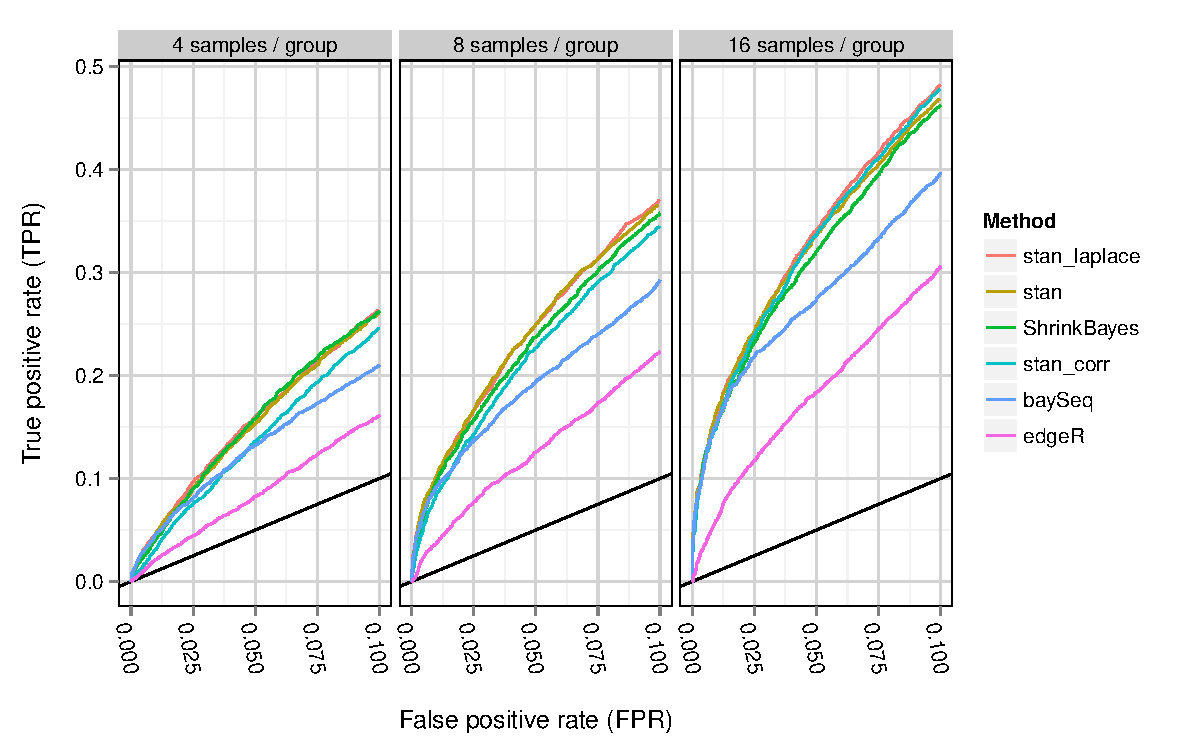
\includegraphics[width=0.8\textwidth]{exampleROC0_1}}
\caption{Example ROC curves for the first simulation}
\label{f:roc}
\end{figure}

\begin{figure}
\centerline{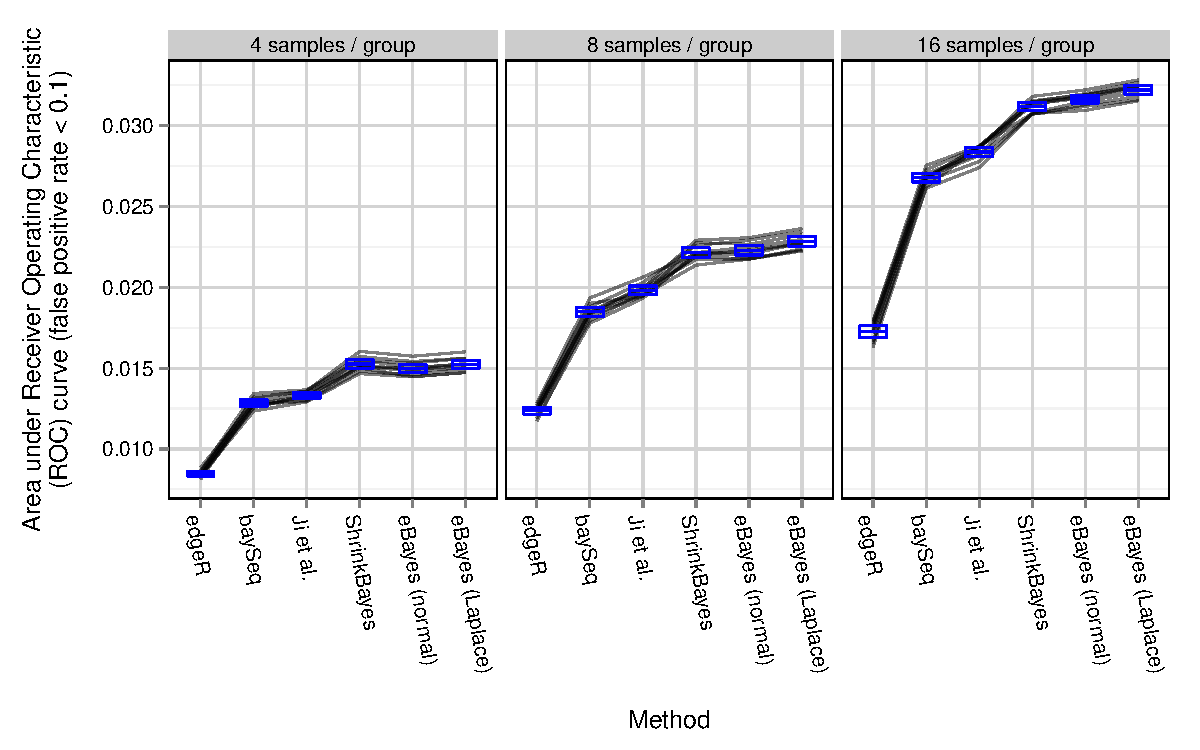
\includegraphics[width=0.8\textwidth]{auc-facet-TRUE}}
\caption{Area under the ROC curves (AUC) for 3 different sample sizes (facets) for the methods under comparison for false positive rates below 0.1. Each line is a different simulation while the blue box indicates mean AUC and its standard error across the simulations.}
\end{figure}

\section{Heterosis in corn ??}
\label{s:corn}

\section{Discussion}
\label{s:discuss}

Put your final comments here. 



\backmatter %  Please keep this command in your document in this position 



\section*{Acknowledgements}

The authors thank Andrew Lithio for help implementing our model in {\tt ShrinkBayes}.

%  If your paper refers to supplementary web material, then you MUST
%  include this section!!  See Instructions for Authors at the journal
%  website http://www.biometrics.tibs.org

\section*{Supplementary Materials}


\bibliography{jarad}
\bibliographystyle{biom}

\appendix

%  To get the journal style of heading for an appendix, mimic the following.

\section{}
\subsection{Stan model for heterosis}



\label{lastpage}

\end{document}
